%\setbeamercolor{background canvas}{bg=yellow!10}

\subtitle{Nociones de Meteorología de la Capa Límite}
 \begin{frame}{}
     \maketitle
 \end{frame}

%\begin{frame}{Humedad}{Medidas de contenido de agua}
%    \begin{itemize}
%    \item Volume Mixing Ratio ($\chi_v$)
%    $$\chi_v =\dfrac{N_q}{N_d}$$
%    \item Mixing Ratio ($\omega_v$)\footnote{$\epsilon=R'/R_v=0.622$, donde $R'=R^*/m_d$ y $R_v=R^*/m_v$}
%    $$\omega_v =\dfrac{\rho_v}{\rho_d}=\epsilon\chi_v$$
%    \item Mass density ($q_v$)
%    $$q_v=\dfrac{\rho_v}{\rho}=\dfrac{\rho_v}{\rho_d + \rho_v}=\dfrac{\omega_v}{1+\omega_v}$$
%    \item Humedad relativa (RH)
%    %\item Dewpoint Depression
%    %\item Saturation Vapor Pressure (es)
%    %\item Vapor Pressure (e)
%    \end{itemize}
%\end{frame}
 
%\begin{frame}{Temperatura Virtual}
%    
%    Es la temperatura que debiera tener el aire seco para tener la misma densidad que el aire con cierta cantidad de humedad.
%    
%    $$\Bigg\rho_{\text{Aire Seco}}   \quad > \quad \Bigg\rho_{\text{Aire húmedo}}$$
%    
%    Peso molecular del aire:
%    $$ m_a = \dfrac{m_d}{1+ 0.608\,q_v }$$ 
%\end{frame}

\begin{frame}{Estructura de la atmósfera}
    \begin{center}
    \begin{tikzpicture}[scale=1.0]
    \begin{axis}[height=8cm, width=5.5cm,
    xlabel=Temperatura ($^\circ$C), 
    ylabel=Altitud (km), ymin=0 ,ymax=110,xmin=-100,xmax=100]%,clip=false]
   
    \draw[fill,pattern color=orange!80,pattern=north east lines,draw=none,minimum width=0.3,minimum height=0] (-100,0) rectangle (100,11);
   
   \node[orange  ] at (50, 5) {Tropósfera};
   \node[black!80] at (50,30) {Estratósfera};
   \node[black!80] at (50,65) {Mesósfera};
   \node[black!80] at (50,95){Termósfera};
   
    \addplot[blue!80,very thick,domain=0:11]  (-6.5*x + 15, x);
    \addplot[blue!80,very thick,domain=11:20] (-56.65, x);
    \addplot[blue!80,very thick,domain=20:32] (-56.65+ 1*(x-20) , x);  %stratosfera
    \addplot[blue!80,very thick,domain=32:47] (-44.5+ 2.8*(x-32) , x); %stratosfera
    \addplot[blue!80,very thick,domain=47:55] ( -2.5, x);
    \addplot[blue!80,very thick,domain=55:80] (-3.08*x+166 , x);
    \addplot[blue!80,very thick,domain=80:90] (-80, x);
    \addplot[blue!80,very thick,domain=90:115] (4.66*x-500, x);
    
    \draw[dashed] (-100,11)--(30,11) node[right]{\tiny Tropopausa};
    \draw[dashed] (-100,50)--(30,50) node[right]{\tiny Estratopausa};
    \draw[dashed] (-100,80)--(30,80) node[right]{\tiny Mesopausa};
    
    \end{axis}
    \end{tikzpicture}
    \end{center}
\end{frame}

\begin{frame}{Capa límite Planetaria}

Los fenómenos vinculados al transporte de contaminantes tiene lugar en la \alert{capa limite planetaria} (CLP)
    \begin{center}
    \begin{tikzpicture}[scale=1.3]
    \clip(-4,-0.3) rectangle (4,1.5);
    
    \draw[thick,fill=blue!5, circle] (-3,0) to[out=30,in=185](-0.5,1.2)to[out=5,in=140] (3.2,0);
    \draw[very thick,fill=blue!20, circle,dashed] (-1.8,0) to[out=30,in=173] (0,0.55) to[out=1,in=155] (1.8,0);
    \draw[thick, circle,fill=white] (-1,0) to[out=31, in=149] (1.1,0);
    \draw[ultra thick, ground, circle] (-1,0) to[out=30, in=150] (1.1,0);
 
    \node[fill=white,inner sep=1pt,ellipse] at (0,0) {Tierra};
    \node[rotate=30] at (-1,0.2) {CLP};
    \node[rotate=2] at (-.2,0.9) {Atm. Libre};
    \node[rotate=37] at (-2,0.1) {Inversion};
    \node[rotate=37] at (-2,-0.2) {$z_i$};
      
      \draw[latex-latex,thick,black!70] (1.1,0)--(1.25,0.3) node[midway,anchor=west,rotate=-30]{\small $2$ km};
      \draw[latex-latex,thick,black!70] (0.8,0.12)--(1.1,1.15) node[midway,anchor=west,rotate=-25]{\small $11$ km (Tropósf.)};
    \end{tikzpicture}
    \end{center}
 
 %Características:
 \begin{itemize} 
    \item Abarca los primeros 1-4km de la tropósfera.
    \item Rápida respuesta a influencia de la superificie (calentamiento y fricción).
    \item Límitada verticalmente por la superficie y la capa de inversión que se forma en contacto con la atmósfera libre.
    \item Turbulenta, y por lo tanto bien mezclada.
 \end{itemize}
%A su vez podemos subdividirla en:
%\begin{itemize}
%    \item \textit{Capa superficial} (100-400m): zona donde la velocidad del viento está influenciada por los elementos de la superficie.
%
%    \item \textit{Capa de mezcla}: la turbulencia es suficiente como para asumir mezclado completo.
%\end{itemize}
\end{frame}

\section{Estabilidad}
\begin{frame}{Estabilidad}{Concepto de estabilidad}

Respuesta de un sistema a perturbaciones:
    \begin{center}
        
    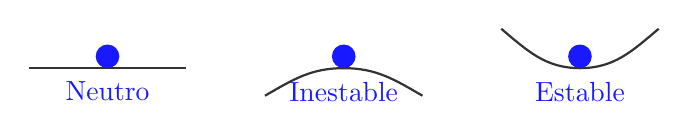
\begin{tikzpicture}
    %NEUTURO:
     \begin{scope}
     %analogia bolitas------------------ 
     \fill[blue!90]  (0,-1) circle (0.15cm) node[anchor=north, yshift=-0.2cm]{Neutro};
     \draw[thick,black!80,yshift=-0.15cm] (-1,-1) -- (1,-1);
     %---------------------------------- 
     \end{scope} 
    %INESTABLE:
     \begin{scope}[xshift=3cm]
     %analogia bolitas ----------------
     \fill[blue!90]  (0,-1) circle (0.15cm) node[anchor=north, yshift=-0.2cm]{Inestable};
     \draw[thick,black!80,yshift=-0.15cm] (-1,-1.35) to[out=30,in=180] (0,-1) to [out=0,in=150] (1,-1.35);
     %---------------------------------- 
     \end{scope} 
     %ESTABLE:
     \begin{scope}[xshift=6cm]
     %Analogia bolitas------------------ 
     \fill[blue!90]  (0,-1) circle (0.15cm) node[anchor=north,yshift=-0.2cm]{Estable};
     \draw[thick,black!80,yshift=-0.15cm] (-1,-0.5) to[out=-40,in=180] (0,-1) to [out=0,in=220] (1,-0.5);
     %---------------------------------- 
     \end{scope} 
    \end{tikzpicture}
    \end{center}
    
    \pause
    
    Aplicado al transporte de contaminantes:
    \begin{center}
    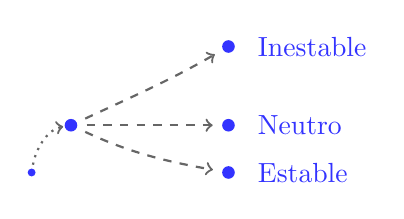
\begin{tikzpicture}
      \ejesXZ{-5}{0}{0.45}
      \piso{-4}{3.0}{0}
      \chimenea{-3.1}{0}{0.2}{1.2}
      
    \coordinate (O) at (-3.0,1.4); %original
    \coordinate (P) at (-2.5,2.0); %perturbada
    \coordinate (E) at (-0.5,1.4); %estable
    \coordinate (N) at (-0.5,2.0); %neutro
    \coordinate (I) at (-0.5,3.0); %inestable
     
     \draw[->, dotted, thick,black!60, shorten <=0.1cm,, shorten >=0.1cm] (O) to[out= 80,in=190] (P);
     \draw[->, dashed, thick,black!60, shorten <=0.2cm,, shorten >=0.2cm] (P) to[out=-25,in=170] (E);
     \draw[->, dashed, thick,black!60, shorten <=0.2cm,, shorten >=0.2cm] (P) to[out=  0,in=180] (N);
     \draw[->, dashed, thick,black!60, shorten <=0.2cm,, shorten >=0.2cm] (P) to[out= 25,in=210] (I);
    
    \fill[blue!80]  (O) circle (0.05cm);
    \fill[blue!80]  (P) circle (0.08cm);
    \fill[blue!80]  (E) circle (0.08cm) node [anchor=west,xshift=0.25cm]{Estable};
    \fill[blue!80]  (N) circle (0.08cm) node [anchor=west,xshift=0.25cm]{Neutro};
    \fill[blue!80]  (I) circle (0.08cm) node [anchor=west,xshift=0.25cm]{Inestable};
    \end{tikzpicture}
    \end{center}
\end{frame}

\begin{frame}{Estabilidad}{Gradiente adiabatico seco}
 
 
Definimos al \alert{gradiente adiabático seco} como la tasa a la que cambia la temperatura de un volumen de aire en respuesta a la compresión/expansión asociada a un cambio de altura, bajo el supuesto de que ocurre de forma adiabática. 
 
$$\Gamma= -\dfrac{dT}{dz} $$
 
 Se puede demostrar que:  \footnote{Utilizando $d Q = 0 = dU + dW = mC_pdT - dp V$ y $dp = \rho g dz$. Donde: $g\approx-9.81 m\,s^{-2}$ y $C_p\approx 1003.5\, J(kg\,K)^{-1}$} 
$$\Gamma=  \dfrac{g}{C_p}\approx  9.75 \, ^\circ K/km $$
    
    
    %    The adiabatic lapse rate is the rate at which the temperature of an air parcel changes in response to the compression or expansion associated with elevation change, under the assumption that the process is adiabatic, i.e., no heat exchange occurs between the given air parcel and its surroundings
% Para una parcela de aire húmeda, el \alert{gradiente adiabático húmedo}:
% $$ \Gamma _{\text{w}}=g\,{\frac {\left(1+{\dfrac {H_{\text{v}}\,r}{R_{\text{sd}}\,T}}\right)}{\left(c_{\text{pd}}+{\dfrac {H_{\text{v}}^{2}\,r}{R_{\text{sw}}\,T^{2}}}\right)}}=g\,{\dfrac {R_{\text{sd}}\,T^{2}+H_{\text{v}}\,r\,T}{c_{\text{pd}}\,R_{\text{sd}}\,T^{2}+H_{\text{v}}^{2}\,r\,\epsilon }}$$
\end{frame}


\begin{frame}{Estabilidad}{Respuesta a perturbaciónes verticales}
    
 Dependiendo del perfil de temperaturas, al perturbar verticalmente una parcela de aire, pueden ocurrir las siguientes situaciones:
\begin{center}
\begin{tikzpicture}[scale=0.8]
    \begin{axis}[xshift=9cm,%no markers,
     samples=5,axis lines*=left, 
     xlabel=T, ylabel=z,
     height=5cm, width=3.5cm,
     xmin=-60,xmax=50, ymin=0  ,ymax=5,
     %xtick=\empty, ytick=\empty,
     enlargelimits=false, 
     ]%
       \addplot [very thick,dashed] (- 9.8*x + 30, x);%grad adiab seco
       \addplot [very thick,red!80     ] (- 2.0*x + 20, x);  % Neutro
       \addplot [very thick,blue       ] (-18.0*x + 40, x);  % Inestable
       \addplot [very thick,red!50!blue] (-10.0*x + 30, x);  %Estable
        
       \draw[black!80, fill=red!50]       (18,1.2) circle (0.1cm);
       \draw[black!80, fill=red!50!blue]  (-9 ,4.0) circle (0.15cm);
    \end{axis}

    \begin{scope}
    \piso{-1.2}{1.2}{0}
    %abajo
    \fill[top color=red!50!blue, middle color=red!50, bottom color=red!50] (-1.2,0) rectangle (1.2,3.7);
    \fill[pattern=my crosshatch dots,pattern color=red!50] (-1.2,0) rectangle (1.2,2);
    %\fill[pattern=my crosshatch dots,pattern color=red!50]  (0,1) circle (0.3cm);
    \fill[red!50]  (0,1) coordinate(A) circle (0.3cm);
    %\draw[very thick, red!50] (0,1) circle (0.3cm);
    \draw[dashed, thick, black!80] (0,1) circle (0.3cm);
    %arriba 
    \fill[pattern=my crosshatch dots,pattern color=red!50!blue] (-1.2,2.3) rectangle (1.2,3.7);
    %\fill[pattern=my crosshatch dots, pattern color=red!50!blue]  (0,3) circle (0.5cm);
    \fill[red!50!blue]  (0,3) circle (0.5cm);
    %\draw[very thick, red!50!blue] (0,3) circle (0.5cm);
    \draw[thick,dashed, black!80] (0,3) circle (0.5cm);
 
    \draw[-latex,thick,dotted,black!80](-0.3,1.3)to[out=150,in=220](-0.3,2.5);%node[midway,left]{\small $w'$};
    
    %analogia bolitas------------------ 
    \fill[blue!80]  (0,-1) circle (0.15cm) node[anchor=north, yshift=-0.2cm]{Neutro};
    \draw[thick,black!80,yshift=-0.15cm] (-1,-1) -- (1,-1);
    %---------------------------------- 
    \end{scope}
\pause  
    \begin{scope}[xshift=3cm]
    \piso{-1.2}{1.2}{0}
    %abajo
    \fill[top color=blue!80, middle color=red!50, bottom color=red!50] (-1.2,0) rectangle (1.2,3.7);
     \fill[pattern=my crosshatch dots,pattern color=red!50] (-1.2,0) rectangle (1.2,2);
    
    %\fill[pattern=my crosshatch dots,pattern color=red!50]  (0,1) coordinate(A) circle (0.3cm);
    \fill[red!50]  (0,1) coordinate(A) circle (0.3cm);
    %\draw[very thick, red!50] (0,1) circle (0.3cm);
    \draw[dashed, thick, black!80] (0,1) circle (0.3cm);
    %arriba
    \fill[pattern=my crosshatch dots,pattern color=blue!80] (-1.2,2.3) rectangle (1.2,3.7);
    \fill[pattern=my crosshatch dots,pattern color=red!50!blue]  (0,3) coordinate (B) circle (0.5cm);
    \fill[red!50!blue]  (0,3) coordinate (B) circle (0.5cm);
    %\draw[very thick, red!50!blue] (0,3) circle (0.5cm);
    \draw[thick,dashed, black!80] (0,3) circle (0.5cm);
 
    \draw[-latex,thick,dotted,black!80](-0.3,1.3)to[out=150,in=220](-0.3,2.5);%node[midway,left]{\small $w'$};
    \draw[-latex, ultra thick, black!80] (B) --++(0,1)node[midway,right]{};
    %analogia bolitas ----------------
    \fill[blue!80]  (0,-1) circle (0.15cm) node[anchor=north, yshift=-0.2cm]{Inestable};
    \draw[thick,black!80,yshift=-0.15cm] (-1,-1.35) to[out=30,in=180] (0,-1) to [out=0,in=150] (1,-1.35);
    %---------------------------------- 
    
    \end{scope}
\pause
    \begin{scope}[xshift=6cm]
    \piso{-1.2}{1.2}{0}
    %abajo
    \fill[top color=red!80, middle color=red!50, bottom color=red!50] (-1.2,0) rectangle (1.2,3.7);
    \fill[pattern=my crosshatch dots,pattern color=red!50] (-1.2,0) rectangle (1.2,2);
    
    %\fill[pattern=my crosshatch dots,pattern color=red!50]  (0,1) coordinate(A) circle (0.3cm);
    \fill[red!50]  (0,1) coordinate(A) circle (0.3cm);
    %\draw[very thick, red!50] (0,1) circle (0.3cm);
    \draw[dashed, thick, black!80] (0,1) circle (0.3cm);
    
    %arriba
    \fill[pattern=my crosshatch dots,pattern color=red!80] (-1.2,2.3) rectangle (1.2,3.7);
    %\fill[pattern=my crosshatch dots,pattern color=red!50!blue]  (0,3) coordinate (B) circle (0.5cm);
    \fill[red!50!blue]  (0,3) coordinate (B) circle (0.5cm);
    \draw[thick,dashed, black!80] (0,3) circle (0.5cm);
 
    \draw[-latex,thick,dotted,black!80](-0.3,1.3)to[out=150,in=220](-0.3,2.5);%node[midway,left]{\small $w'$};
    \draw[-latex, ultra thick, black!80] (B) --++(0,-1)node[midway,right]{};
    
    %Analogia bolitas------------------ 
    \fill[blue!80]  (0,-1) circle (0.15cm) node[anchor=north,yshift=-0.2cm]{Estable};
    \draw[thick,black!80,yshift=-0.15cm] (-1,-0.5) to[out=-40,in=180] (0,-1) to [out=0,in=220] (1,-0.5);
    %---------------------------------- 
    
    \end{scope}

\end{tikzpicture}
\end{center}

    RECORDAR: Si una parcela de aire está a mayor temperatura que su entorno entonces asciende.
\end{frame}


\begin{frame}{Estabilidad}{Efecto en el transporte de contaminantes}
\begin{columns}
\column{0.5\textwidth}
\pause
 
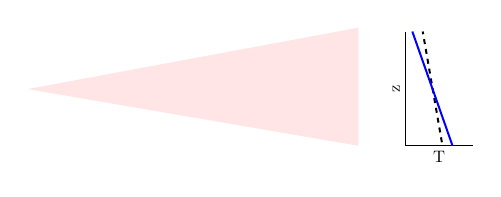
\begin{tikzpicture}[scale=0.6]
\ejesXZ{-5}{0}{0.45}
\piso{-4}{4.5}{0}
\chimenea{-3.1}{0}{0.2}{1.2}
 %pluma real
\fill[red!20,opacity=0.5] (-3,1.2) -- (4,2.5) -- (4,0) -- (-3,1.2);
    \begin{axis}[xshift=5cm,%no markers,
    samples=5,axis lines*=left, xlabel=T, ylabel=z,
    height=4cm, width=3cm,
    xmin=-50,xmax=50, ymin=0  ,ymax=5,
    %x dir=reverse,
    xtick=\empty, ytick=\empty,
    enlargelimits=false, 
    ]%
    \addplot [very thick,dashed] (-5.9*x + 5 ,x);%grad adiab seco
    \addplot [very thick,blue] (-12*x + 20, x);%strong lapse (looping)
    \end{axis}
\end{tikzpicture}

\pause
 
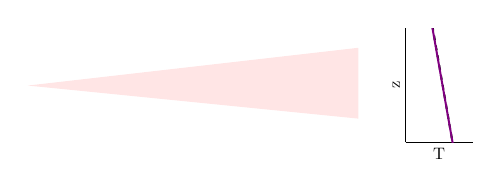
\begin{tikzpicture}[scale=0.6]
\ejesXZ{-5}{0}{0.45}
\piso{-4}{4.5}{0}
\chimenea{-3.1}{0}{0.2}{1.2}
 %pluma real
\fill[red!20,opacity=0.5] (-3,1.2) -- (4,2) -- (4,0.5) -- (-3,1.2);
    \begin{axis}[xshift=5cm,%no markers,
    samples=5,axis lines*=left, xlabel=T, ylabel=z,
    height=4cm, width=3cm,
    xmin=-50,xmax=50, ymin=0  ,ymax=5,
    %x dir=reverse,
    xtick=\empty, ytick=\empty,
    enlargelimits=false, 
    ]%
    \addplot [very thick,dashed] (-5.9*x + 20,x);%grad adiab seco
    \addplot [very thick,red!50!blue] (-6.0*x + 20, x);%weak lapse (conning)
    \end{axis}
\end{tikzpicture}

\pause
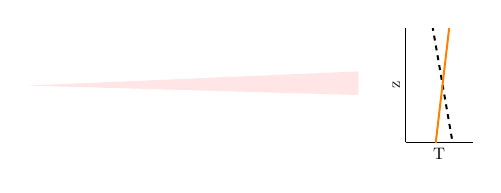
\begin{tikzpicture}[scale=0.6]
\ejesXZ{-5}{0}{0.45}
\piso{-4}{4.5}{0}
\chimenea{-3.1}{0}{0.2}{1.2}
 %pluma real
\fill[red!20,opacity=0.5] (-3,1.2) -- (4,1.5) -- (4,1.0) -- (-3,1.2);
    \begin{axis}[xshift=5cm,%no markers,
    samples=5,axis lines*=left, xlabel=T, ylabel=z,
    height=4cm, width=3cm,
    xmin=-50,xmax=50, ymin=0  ,ymax=5,
    %x dir=reverse,
    xtick=\empty, ytick=\empty,
    enlargelimits=false, 
    ]%
    \addplot [very thick,dashed] (-5.9*x + 20,x);%grad adiab seco
    \addplot [very thick,orange] ( 4*x - 5 , x);%estable (fanning)
    \end{axis}
\end{tikzpicture}
 
\column{0.5\textwidth}
\pause
 
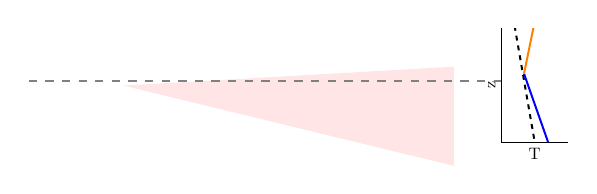
\begin{tikzpicture}[scale=0.6]
    \ejesXZ{-5}{0}{0.45}
    \piso{-4}{4.5}{0}
    \chimenea{-3.1}{0}{0.2}{1.2}
     %pluma real
    \fill[red!20,opacity=0.5] (-3,1.2) -- (4,1.6) -- (4,-0.5) -- (-3,1.2);
    \begin{axis}[xshift=5cm,%no markers,
    samples=5,axis lines*=left, xlabel=T, ylabel=z,
    height=4cm, width=3cm,
    xmin=-50,xmax=50, ymin=0  ,ymax=5,
    %x dir=reverse,
    xtick=\empty, ytick=\empty,
    enlargelimits=false, 
    ]%
    \addplot [very thick,dashed] (-5.9*x -  0,x);%grad adiab seco
    \addplot [very thick,blue,domain=0:3] (-12*x + 20, x);%strong lapse (looping)
    \addplot [very thick,orange,domain=3:6] (7*x -37, x);%strong lapse (looping)
    \end{axis}
    \draw[dashed,thick,gray] (-5,1.3)--(5,1.3);%inversion 
\end{tikzpicture}
\pause
  
 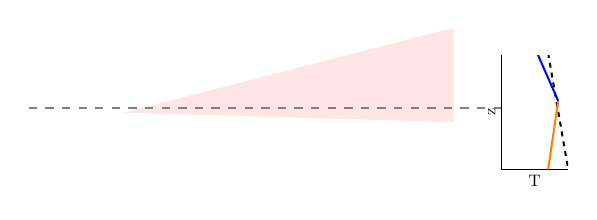
\begin{tikzpicture}[scale=0.6]
     \ejesXZ{-5}{0}{0.45}
     \piso{-4}{4.5}{0}
     \chimenea{-3.1}{0}{0.2}{1.2}
      %pluma real
     \fill[red!20,opacity=0.5] (-3,1.2) -- (4,3) -- (4,1.) -- (-3,1.2);
     \begin{axis}[xshift=5cm,%no markers,
     samples=5,axis lines*=left, xlabel=T, ylabel=z,
     height=4cm, width=3cm,
     xmin=-50,xmax=50, ymin=0  ,ymax=5,
     %x dir=reverse,
     xtick=\empty, ytick=\empty,
     enlargelimits=false, 
     ]%
     \addplot [very thick,dashed] (-5.9*x + 50,x);%grad adiab seco
     \addplot [very thick,orange,domain=0:3] ( 5*x + 20, x);%inversion (fanning)
     \addplot [very thick,blue,domain=3:7] ( -15*x + 80, x);%inversion (fanning)
     \end{axis}
     \draw[dashed,thick,gray] (-5,1.3)--(5,1.3);%inversion 
 \end{tikzpicture}
\pause
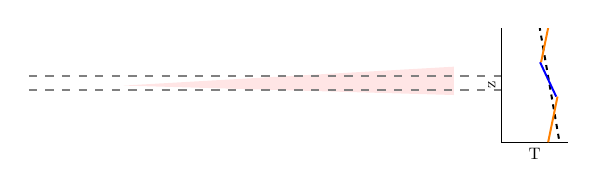
\begin{tikzpicture}[scale=0.6]
    \ejesXZ{-5}{0}{0.45}
    \piso{-4}{4.5}{0}
    \chimenea{-3.1}{0}{0.2}{1.2}
     %pluma real
    \fill[red!20,opacity=0.5] (-3,1.2) -- (4,1.6) -- (4,1) -- (-3,1.2);
    \begin{axis}[xshift=5cm,%no markers,
    samples=5,axis lines*=left, xlabel=T, ylabel=z,
    height=4cm, width=3cm,
    xmin=-50,xmax=50, ymin=0  ,ymax=5,
    %x dir=reverse,
    xtick=\empty, ytick=\empty,
    enlargelimits=false, 
    ]%
    \addplot [very thick,dashed] (-5.9*x + 37,x);%grad adiab seco
    \addplot [very thick,orange,domain=0:2] ( 7.0*x + 20, x);%weak lapse (conning)
    \addplot [very thick,blue ,domain=2:3.5] (-16.0*x + 64, x);%weak lapse (conning)
    \addplot [very thick,orange,domain=3.5:6] ( 7.0*x - 15, x);%weak lapse (conning)
    \end{axis}
    \draw[dashed,thick,gray] (-5,1.4)--(5,1.4);%inversion 
    \draw[dashed,thick,gray] (-5,1.1)--(5,1.1);%inversion 
\end{tikzpicture}
\end{columns}
\end{frame}


  
\begin{frame}{Estabilidad}{Temperatura potencial}
La \alert{temperatura potencial} ($\theta$) es la temperatura que tendría una parcela de aire seca si fuese llevada a $p_0=1000$hPa de forma adiabática. 
$$ \theta = T \bigg( \dfrac{p_0}{p}\bigg)^{R/(c_p M)} $$
 
% También puede pensarse como (informal): la temperatura que tendría una parcela de aire si le devolvemos todo lo que perdió adiabáticamente por estar a la altura que está.
\pause 
Expresado en relación a la altura:
 $$\theta= T - z\, \Gamma  $$
% La \alert{temperatura potencial virtual} ($\theta_v$) es la temperatura que tendría una parcela de aire húmeda si se le extrajera toda su humedad y fuese llevada a $p_0=1000$hPa de forma adiabática . 
%  
% $$ \theta_v = T (1+0.608\,q_v)\bigg( \dfrac{p_0}{p}\bigg)^{R/(c_p M)} $$

\pause

Es más fácil distinguir estabilidad gráficamente si usamos $\theta$:
\begin{center}
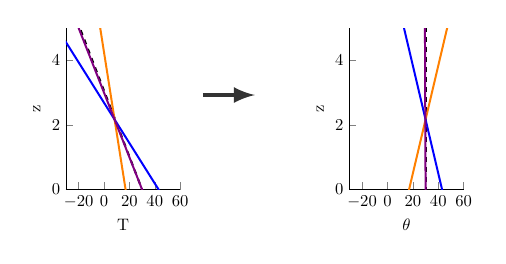
\begin{tikzpicture}[scale=0.6]
  
\begin{scope}[xshift=-3cm]
\begin{axis}[%no markers,
 samples=5,axis lines*=left, 
 xlabel=T, ylabel=z,
 height=5cm, width=4cm,
 xmin=-30,xmax=60, ymin=0  ,ymax=5,
 %xtick=\empty, ytick=\empty,
 enlargelimits=false, 
 ]%
 \addplot [very thick,dashed] (- 9.8*x + 30, x);%grad adiab seco
 \addplot [very thick,orange ] (- 4.0*x + 17, x);%weak lapse (conning)
 \addplot [very thick,blue  ] (-16.0*x + 43, x);%weak lapse (conning)
 \addplot [very thick,red!50!blue  ] (-10.0*x + 30, x);%weak lapse (conning)
 \end{axis}
\end{scope}

\pause 
\draw[-latex, ultra thick,black!80] (-0.1,2)--(1.0,2);

\begin{scope}[xshift=3cm]
\begin{axis}[%no markers,
 samples=5,axis lines*=left, 
 xlabel=$\theta$, ylabel=z,
 height=5cm, width=4.0cm,
 xmin=-30,xmax=60, ymin=0  ,ymax=5,
 %xtick=\empty, ytick=\empty,
 enlargelimits=false, 
 ]%
 \addplot [very thick,dashed] (- 0*x + 30, x);%grad adiab seco
 \addplot [very thick,orange ] (  6.0*x + 17, x);       %weak lapse (conning)
 \addplot [very thick,blue  ] (- 6.0*x + 43, x);       %weak lapse (conning)
 \addplot [very thick,red!50!blue  ] (-0.1*x + 30, x);%weak lapse (conning)
 \end{axis}
\end{scope}

\end{tikzpicture}
\end{center}

\end{frame}


\begin{frame}{Estabilidad}{Indicadores de estabilidad}
    
    Llamemos $\Lambda$ al \alert{gradiente de temperatura real}, podemos determinar la estabilidad atmosférica según:
    
    $$\Lambda \begin{cases}
        <\Gamma & \text{(estable/sub-adiabatico)}\\
        =\Gamma & \text{(neutral)} \\
        >\Gamma & \text{(inestable/super-adiabatico)} \\
    \end{cases}$$

%\pause

%También se puede determinar la estabilidad en base a la \alert{temperatura potencial}:
%    $$\dfrac{d\theta}{dz} \begin{cases}
%        <0 & \text{(inestable)}\\
%        =0 & \text{(neutral)} \\
%        >0 & \text{(estable)} \\
%    \end{cases}$$
    
\end{frame}
  
%\begin{frame}{Estabilidad}{Parámetro de estabilidad}
%Expresa la tendencia de una parcela de aire a acelerarse en contra de movimientos verticales.
%\footnote{
%$F= \rho V a =  (\rho-\rho_a)V g  \quad \Rightarrow \quad a = g(\rho-\rho_a)/\rho$. 
%Usando la ley de los gases ideales:
%$a = g(T_a -T) /T_a$, finalmente dividimos por $dz$ y $a= g(\Gamma -\Lambda) /T_a$. Usando la definicion de temperatura potencial: $d\theta/dz =  (\Gamma - \Lambda)$
%}
%$$s=a=\dfrac{\Gamma - \Lambda}{T_a}g = \dfrac{g}{T_a}\dfrac{d\theta}{dz}$$
%\end{frame}
  

\section{Balance de energía superficie-atmósfera}
 
\begin{frame}{Balance de energía}{Cálculo de calor sensible \footnote{ $R_n$: radiación neta. $H$: flujo de calor sensible. $L$: flujo de calor latente. $G$: flujo de calor al suelo. Los signos del balance están planteado a favor de la atmósfera.}}
 
\begin{center}
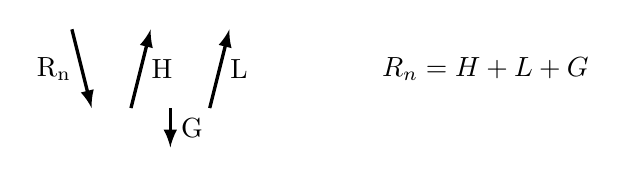
\begin{tikzpicture}[scale=0.5]
    \begin{scope}
    \piso{-3}{3}{0}
    \draw[-latex,very thick] (-2.5, 2.0) -- (-2.0, 0.0) node[midway,anchor=east]{$\mathrm{R_n}$} ;
    \draw[-latex,very thick] (-1.0, 0.0) -- (-0.5, 2.0) node[midway,anchor=west]{$\mathrm{H}$  };
    \draw[-latex,very thick] ( 0.0, 0.0) -- ( 0.0,-1.0) node[midway,anchor=west]{$\mathrm{G}$  };
    \draw[-latex,very thick] ( 1.0, 0.0) -- ( 1.5, 2.0) node[midway,anchor=west]{$\mathrm{L}$  };
    \end{scope}
   
    \node at (8,1) {$R_n = H + L + G$};
\end{tikzpicture}
\end{center}
\vspace{-0.5em}
 
\pause
Considerando:\footnote{$B_0$: Relación de Bowen, depende de la humedad disponible en el tipo de cobertura.}
$$ G \approx 0.1 R_n \qquad B_0 =\dfrac{H}{L}  $$

\pause 
El calor sensible (H) se puede calcular como:
$$ 
H = \dfrac{0.9\,R_n}{ 1 + 1/B_0}
\qquad
\begin{cases}
    H>0  & \text{Flujo atmosfera a superifice (ESTABLE)}  \\
    H=0  & \text{No hay flujo neto (NEUTRO)}  \\
    H<0  & \text{Flujo superficie a atmosfera (INESTABLE)}
\end{cases}
$$
\end{frame}
 
\begin{frame}{Balance Radiativo}{Radiación Neta}
 
 Separamos lo que es onda larga ó infraroja (IR) de onda corta ó visible (V):
\footnote{$a_o$: albedo. $\sigma_{SB}$: cte. Stephan-Boltzman. $n$: fracciòn nubosa. $c_1$ y $c_2$: constantes empìricas.} 

    $$
    R_n  
    =
    \underbrace{R}_{V\downarrow}
    -
    \underbrace{a_o\,R}_{V\uparrow}
    -
    \underbrace{\varepsilon\,\sigma_{SB}T_s^4}_{IR\uparrow}
    +
    \underbrace{c_1\,T_a^6 + c_2\,n}_{IR\downarrow}
    $$

\pause      
 
\begin{center}
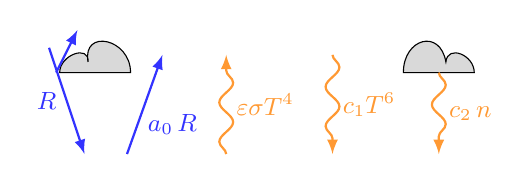
\begin{tikzpicture}[scale=0.9,
    %waveVIS/.style={decorate, decoration=snake,amplitude=0.01mm, segment length=2.5mm},
    waveIR/.style ={decorate, decoration=snake,segment length=5mm}]
  \begin{scope}
  \piso{-3}{3}{0}
 
 \draw[fill=gray!30] (2,1.25) to[out=90,in=100,looseness=2] (2.6,1.4) to[out=85,in=90,looseness=1.5] (3,1.25) -- cycle;
 \draw[fill=gray!30,xshift=-0.85cm] (-1,1.25) to[out=90,in=100,looseness=2] (-1.6,1.4) to[out=85,in=90,looseness=1.5] (-2,1.25) -- cycle;
 
  \draw[-latex,thick,blue!80] (-3.0, 1.6) -- (-2.5, 0.1) node[midway,anchor=east]{\small$R$} ;
  \draw[-latex,thick,blue!80] (-2.9, 1.25)--++(.3, 0.6) node[midway,anchor=west]{};
  \draw[-latex,thick,blue!80] (-1.9, 0.1) -- (-1.4, 1.5) node[midway,anchor=west,pos=0.3]{\small$a_0\,R$};
  \draw[-latex,thick,orange!80,waveIR] (-0.5, 0.1) -- (-0.5, 1.5) node[midway,anchor=west]{\small$\varepsilon\sigma T^4$};
  \draw[-latex,thick,orange!80,waveIR] (1.0, 1.5) -- (1.0, 0.1) node[midway,anchor=west]{\small$c_1T^6$};
  \draw[-latex,thick,orange!80,waveIR] ( 2.5, 1.25) -- ( 2.5, 0.1) node[midway,anchor=west]{\small$c_2\,n$};
  \end{scope}
\end{tikzpicture}
\end{center}

\pause      
 donde R es la radiaciòn incidente:\footnote{$S_o\approx1366 \pm 7 W/m^2$: cte. Solar. $\tau$: transmisividad de la atmos, depende del recorrido de los rayos (i.e la latitud) y de la nubosidad.}
 $$ R= S_o\,\tau_s\,\sin\alpha_s $$
 
\end{frame}





\begin{frame}{Balance Radiativo}{Angulo solar ($\alpha_s$)}

Es el ángulo que forma que forma el sol con respecto al horizonte, y se calcula: \footnote{$\Phi$: latitud, $\delta_s$: declinación solar, $h$: ángulo horario. $h=2\pi\,t / 24 + \lambda$, donde $\lambda$: longitud, y $t$ es la hora global (UTC) del día. $\delta_s=\varphi_t\,\cos 2\pi(d-d_r)/365$, donde $\varphi$: es el angulo del eje terrestre (23.44). }
 $$\sin \alpha_{s}=\sin \Phi \sin \delta_s +\cos \Phi \cos \delta_s \cos h $$%\cos \theta _{s}=


\begin{center}
    
\begin{tikzpicture}[font=\sffamily,scale=0.6]
\tdplotsetmaincoords{70}{210}
\begin{scope}[tdplot_main_coords]
  \draw[fill=blue!10] (3,3,0) -- (3,-3,0) --  (-3,-3,0) -- (-3,3,0) -- cycle;
  \draw[-latex,black!70] (0,0,0) -- (2,0,0) node[pos=1.1] {$x$};
  \draw[-latex,black!70] (0,0,0) -- (0,2,0) node[pos=1.1] {$y$};
  \draw[-latex,black!70] (0,0,0) -- (0,0,2) node[pos=1.1] {$z$};
  %
  \draw[dashed] (0,0,0) -- (0,0,4) -- (1,2,4) coordinate (O)-- (1,2,0) -- (0,0,0);
  \draw[-latex] (0,0,0) -- (O) node[pos=1.03,circle,inner sep=1pt,fill,label=above left:$Sol$]{};
  %
  \tdplotdefinepoints(0,0,0)(1,2,0)(1,2,4)
  \tdplotdrawpolytopearc[thick,-latex,orange]{1.5}{anchor=west,orange}{$\alpha_s$}
  %\tdplotdefinepoints(0,0,0)(1,0,4)(1,2,4)
  %\tdplotdrawpolytopearc[thick,-latex,purple]{1.5}{anchor=south,purple}{$\theta_s$}
\end{scope}
\end{tikzpicture}
\end{center}

\end{frame}

 
 
 \section{Ciclo Diruno de la CLP}
 \begin{frame}{Ciclo diurno de la CLP}
     
     Evolución en el día de la capa límite:\footnote{donde: CM: Capa de mezcla (Inestable), CE: Capa estable, CR: Capa Residual y CS: Capa de Superficie.}
     \begin{center}
     \begin{tikzpicture}[scale=0.5,yscale=2]
         \CicloDiurnoPBL
     
     \end{tikzpicture}
     \end{center}
     
 \end{frame}
 
 
\section{Temperatura}
 
\begin{frame}{Temperatura}{Ciclo diurno del Flujo de calor sensible}
 
La inversión sobre la CLP actua como una tapa que atrapa el calor generado en la superficie, modificando la temperatura del perfil. La integral en el tiempo del flujo de calor sensible (H), nos da el calor total ($Q_H$) acumulado en la capa límite.
    
    \begin{center}
    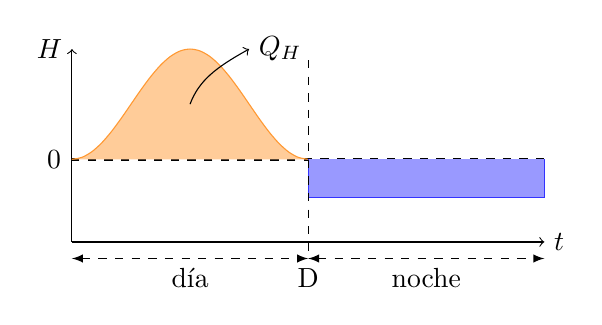
\begin{tikzpicture}[xscale=1.5,yscale=0.7]
    \draw[->] (0,-1.5) -- (4, -1.5) node[right] {$t$};
    \draw[-,dashed,very thick] (4,0) -- (0, 0) node[anchor=east]{0};
    \draw[->] (0,-1.5) -- (0,2) node[left] {$H$};
    \draw[domain=0:2, smooth, variable=\x, orange!80,fill=orange!40 ] plot ({\x}, {1-cos(deg(\x)*3.14/1)});
    \draw[blue!80,fill=blue!40] (2,0)--(2,-0.7)--(4,-0.7)--(4,0);
    
    \draw[dashed] (2,1.8)--(2,-1.8)node[below]{D};
    
    \draw[latex-latex,dashed] (0,-1.8)--(2,-1.8)node[midway,anchor=north]{día};
    \draw[latex-latex,dashed] (2,-1.8)--(4,-1.8)node[midway,anchor=north]{noche};
    
    \draw[->] (1,1.0) to[out=80, in=230] (1.5,2.0) node[right]{$Q_H$};
    \end{tikzpicture}
    \end{center}
    
Para capas estables $\theta$ decrece aproximadamente exponencial con la alturas, mientras que en capas de mezcladas $\theta$ puede considerarse constante en todo el perfil.

\end{frame}


\begin{frame}{Temperatura potencial y altura de capa de mezcla}
    
    Podemos estimar la temperatura potencial en la capa de mezcla considerando el sondeo de temperatura potencial de la mañana y el calor sensible acumulado durante el día. 
    
    \begin{center}
    \begin{tikzpicture}[scale=1.2]

    \begin{scope}[xshift=-1.5cm]
    \draw[->,xshift=0,thick](0,0)--(1.5,0) node[anchor=north]{$t$};
    \draw[->,xshift=0,thick](0,0)--(0,2) node[anchor=east]{$H$};
     
    \draw [orange,very thick]  plot[domain=0:1.5, samples=20] (\x, {0.7*(1+cos(180+180*\x))});
    \fill [ground, pattern color=orange!90]  plot[domain=0:0.7, samples=20] (\x, {0.7*(1+cos(180+180*\x))})--(0.7,0)--cycle;
    
    \draw[very thick, dashed] (0.7,1)--(0.7,0) node[anchor=north]{$t_1$};
    \draw[dotted, black] (0.7,1)--(0,1) node[anchor=east]{$H({t_1})$};
    \end{scope}
     \begin{scope}[xshift=1.5cm]
      \draw[->,xshift=0,thick](0,0)--(1,0) node[anchor=north]{$\theta$};
      \draw[->,xshift=0,thick](0,0)--(0,2) node[anchor=east]{$z$};
      
    %\draw [dashed,very thick,black!90]   plot [domain=0:1.1, samples=20] (\x,\x*\x);
    %\fill [black!80,ground]  plot[domain=0:1,variable=\x] (\x,\x*\x) --(1,0)--(0,0) -- cycle;
    
    \draw[orange,very thick] (0,0)to[out=60,in=260](0.5,1.0)to[out=85,in=240](1,1.7) to[out=90,in=-45](0.8,2);
    \fill[ground, pattern color=orange!60] (0,0)to[out=60,in=260](0.5,1.0) --(0.5,0)--cycle;
    
    \draw[very thick, dashed] (0.5,1)--(0.5,0) node[anchor=north]{$\theta_{\text{mix}}$};
    \draw[dotted, black] (0.5,1)--(0,1) node[anchor=east]{$z_{\text{mix}}$};
    
    \draw[-latex] (0.3,0.2) --(0.7,0.5) node[anchor=west]{\small $\theta_{\text{mix}}\,z_{\text{mix}}- \int_0^{z_{\text{mix}}} \theta(z)\,dz$};
    \end{scope}

    \end{tikzpicture}
    \end{center}
    
    También hay transferencia de calor desde arriba de la capa límite ($\approx 40$\% del calor sensible de la superficie):
    
     $$
     1.4 \int_{t_{\text{amanecer}}}^t H(t) \,dt = c_p \rho\, \bigg[\int_z^{z_{\text{mix.}}} \theta(z_{mix}) - \theta(z) dz \bigg]
     $$
    
    Esta metodología también nos permite conocer la altura de capa de mezcla $z_i$.
\end{frame}

%\begin{frame}{Temperatura en la CLP}{Perfiles de temperatura}
%
%\begin{columns}
%\column{0.5\textwidth}
%Perfiles de temperatura en la CLP:
%\begin{center}
%    \includegraphics[width=\textwidth]{img/PBL_temp.png}
%\end{center}
% 
%\column{0.5\textwidth}
% Perfiles en capa de superficie:
% \begin{center}
%     \includegraphics[width=\textwidth]{img/SL_temp.png}
% \end{center}   
%\end{columns}
%\end{frame}


\begin{frame}{Ciclo diurno de la CLP}{Perfiles de temperatura potencial}
Evolución típica de perfil de temperatura potencial en la CLP:
\begin{center}
   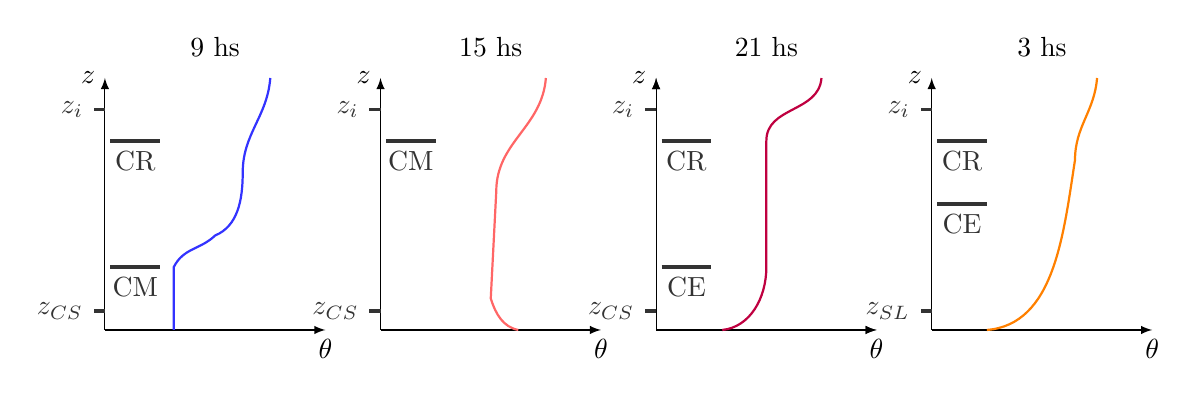
\begin{tikzpicture}[yscale=0.8,xscale=0.7]
        \begin{scope}[xshift=-10cm]
            %General
            \draw[-latex] (0,0)--(4,0)node[below]{$\theta$};\draw[-latex] (0,0)--(0,4)node[left]{$z$};
            \draw[very thick,black!80] (0,3.5)--(-0.2, 3.5) node[left]{$z_i$}; \draw[very thick,black!80] (0,0.3)--(-0.2, 0.3) node[left]{$z_{\text{CS}}$};
            \node at (2,4.5){9 hs};
            %9AM
            \draw[blue!80,thick] (1.25,0)--(1.25,1) to[out=60,in=220] (2,1.5) to[out=20,in=270](2.5,2.5)to[out=90,in=265](3,4);  
            %Layers:
            \draw[very thick,black!80] (0.1,1)--(1, 1) node[midway,below]{CM};
            \draw[very thick,black!80] (0.1,3)--(1, 3) node[midway,below]{CR};
        \end{scope}
        \begin{scope}[xshift=-5cm]
            %General
            \draw[-latex] (0,0)--(4,0)node[below]{$\theta$};
            \draw[-latex] (0,0)--(0,4)node[left]{$z$};
            \draw[very thick,black!80] (0,3.5)--(-0.2, 3.5) node[left]{$z_i$}; \draw[very thick,black!80] (0,0.3)--(-0.2, 0.3) node[left]{$z_{\text{CS}}$};
            \node at (2,4.5){15 hs};
            %3PM
            \draw[red!60,thick] (2.5,0) to[out=170,in=290] (2,0.5) -- (2.1,2.2) to[out=90,in=265](3,4);
             %Layers:
             \draw[very thick,black!80] (0.1,3)--(1, 3) node[midway,below]{CM};
        \end{scope}
        \begin{scope}[xshift=0cm]
           %General
           \draw[-latex] (0,0)--(4,0)node[below]{$\theta$};
           \draw[-latex] (0,0)--(0,4)node[left]{$z$};
           \draw[very thick,black!80] (0,3.5)--(-0.2, 3.5) node[left]{$z_i$}; \draw[very thick,black!80] (0,0.3)--(-0.2, 0.3) node[left]{$z_{\text{CS}}$};
           \node at (2,4.5){21 hs};
            \draw[-latex] (0,0)--(4,0);\draw[-latex] (0,0)--(0,4);
            %9PM: 
            \draw[purple,thick] (1.2,0) to[out=5,in=270] (2,1) to[out=90,in=270] (2,3)to[out=90,in=265](3,4);
             %Layers:
             \draw[very thick,black!80] (0.1,1)--(1, 1) node[midway,below]{CE};
             \draw[very thick,black!80] (0.1,3)--(1, 3) node[midway,below]{CR};
        \end{scope}
        \begin{scope}[xshift=5cm]
             %General
             \draw[-latex] (0,0)--(4,0)node[below]{$\theta$};
             \draw[-latex] (0,0)--(0,4)node[left]{$z$};
             \draw[very thick,black!80] (0,3.5)--(-0.2, 3.5) node[left]{$z_i$}; \draw[very thick,black!80] (0,0.3)--(-0.2, 0.3) node[left]{$z_{\text{SL}}$};
             \node at (2,4.5){3 hs};
            %3PM
            \draw[orange,thick] (1,0) to[out=4, in=260] (2.6,2.7) to[out=90,in=265] (3,4);
             %Layers:
             \draw[very thick,black!80] (0.1,2)--(1, 2) node[midway,below]{CE};
             \draw[very thick,black!80] (0.1,3)--(1, 3) node[midway,below]{CR};
        \end{scope}
   \end{tikzpicture}   
\end{center}
\end{frame}

\section{Velocidad del Viento}

\begin{frame}{Viento de Superficie}

Por encima de la CLP tenemos viento geostrófico:\footnote{$\text{FGP}=- \nabla p / \rho$ \& $F_{\text{Coriolis}}=-2 (\Omega \times \vec{v})$ }

\begin{center}
\begin{tikzpicture}[scale=1.0]
%Viento geostrófico
\begin{scope}[xshift=-3cm]
\node at (2,3.3){Viento Geostrófico};
  \node[rotate=90] at (-0.3, 1.5){\small Lat.};
  \node[rotate= 0] at ( 2.0,-0.3){\small Lon.};
  
  \clip (0,0) rectangle (4,3);
  \draw[very thick] (0,0) rectangle (4,3);
  \foreach \x in {-0.5,0,0.5,...,2}  \draw[thin,dashed,blue!80] (0,\x) to[out=0, in=180] (4,{\x+1.5});
  \node[red ] at (0.5,2.6){\textbf{A}};
  \node[blue] at (3.5,0.3){\textbf{B}};

  \coordinate (C) at (2.0,1.5);
  \fill[orange!80] (C) circle (0.1cm);
  
  \draw[-latex,  very thick,black!70 ] (C)--++(-0.5, 1.0) node[right]{\small Coriolis};
  \draw[-latex,  very thick,black!70 ] (C)--++( 0.5,-1.0) node[left ]{\small FGP};
  \draw[-latex, ultra thick,orange!70   ] (C)--++( 0.7, 0.5) node[below]{\small \vec{u}};
\end{scope}

\pause
%Viento de superficie
\begin{scope}[xshift= 3cm]
\node at (2,3.3){Viento de Superficie};
  \node[rotate=90] at (-0.3, 1.5){\small Lat.};
  \node[rotate= 0] at ( 2.0,-0.3){\small Lon.};
  
  \clip (0,0) rectangle (4,3);
  \draw[very thick] (0,0) rectangle (4,3);
  \foreach \x in {-0.5,0,0.5,...,2}  \draw[thin,dashed,blue!80] (0,\x) to[out=0, in=180] (4,{\x+1.5});
  \node[red ] at (0.5,2.6){\textbf{A}};
  \node[blue] at (3.5,0.3){\textbf{B}};
 
  \coordinate (C) at (2.0,1.5);
  \fill[orange!80] (C) circle (0.1cm);
  
  \draw[-latex,  very thick,black!70 ] (C)--++( 0.5,-1.0)   node[left ]{\small FGP};
  \draw[-latex,  very thick,black!70 ] (C)--++( 0.2, 1.0)   node[right]{\small Coriolis};
  \draw[-latex,  very thick,purple!70] (C)--++(-0.75, 0.15) node[above]{\small Fricción};
  \draw[-latex, ultra thick,orange!70] (C)--++( 0.5,-0.1)   node[right]{\small \vec{u}};
\end{scope}

\end{tikzpicture}
\end{center}

En la CLP las fuerzas de fricción y la turbulencia hacen que el viento sea más lento (\textit{subgeostrófico}) y se lo suele llamar \alert{viento de superficie}

\end{frame}


\begin{frame}{Ciclo diruno de la CLP}{Perfiles de velocidad del viento}

%Figura 18.18 Stull
\begin{center}
   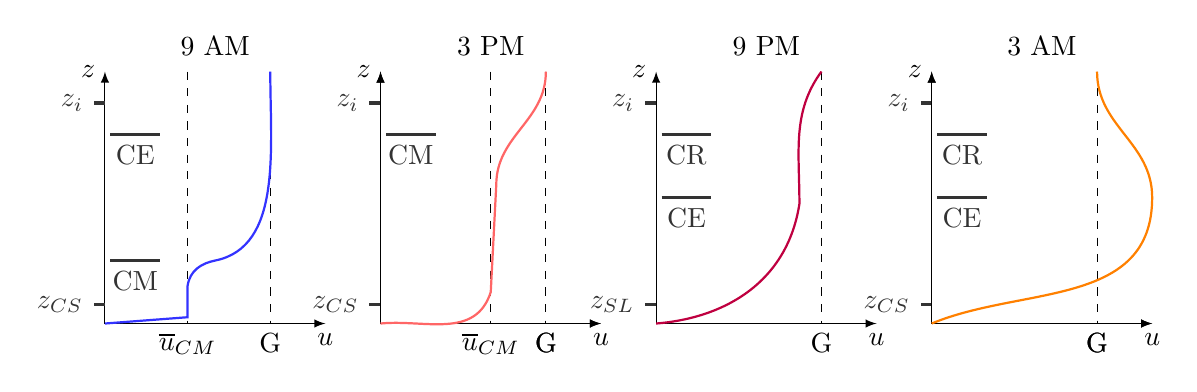
\begin{tikzpicture}[yscale=0.8,xscale=0.7]
        %\draw[-latex] (0,0)--(4,0);\draw[-latex] (0,0)--(0,4);\draw[dashed] (3,4)--(3,0) node[anchor=north]{G};
        
        \begin{scope}[xshift=-10cm]
            %General
            \draw[-latex] (0,0)--(4,0)node[below]{$u$};\draw[-latex] (0,0)--(0,4)node[left]{$z$};\draw[dashed] (3,4)--(3,0) node[anchor=north]{G};
            \draw[very thick,black!80] (0,3.5)--(-0.2, 3.5) node[left]{$z_i$}; \draw[very thick,black!80] (0,0.3)--(-0.2, 0.3) node[left]{$z_{\text{CS}}$};
            \node at (2,4.4){9 AM};
            %Velocidad ML:
            \draw[dashed] (1.5,4)--(1.5,0) node[anchor=north]{$\overline{u}_{CM}$};
            %9AM
            \draw[blue!80,thick] (0,0) -- (1.5,0.1)--(1.5,0.6) to[out=80,in=190] (2,1) to[out=10,in=270](3,4);  
            %Layers:
            \draw[very thick,black!80] (0.1,1)--(1, 1) node[midway,below]{CM};
            \draw[very thick,black!80] (0.1,3)--(1, 3) node[midway,below]{CE};
        \end{scope}
        \begin{scope}[xshift=-5cm]
            %General
            \draw[-latex] (0,0)--(4,0)node[below]{$u$};\draw[-latex] (0,0)--(0,4)node[left]{$z$};\draw[dashed] (3,4)--(3,0) node[anchor=north]{G};
            \draw[very thick,black!80] (0,3.5)--(-0.2, 3.5) node[left]{$z_i$}; \draw[very thick,black!80] (0,0.3)--(-0.2, 0.3) node[left]{$z_{\text{CS}}$};
            \node at (2,4.4){3 PM};
            %G y uML
            \draw[-latex] (0,0)--(4,0);\draw[-latex] (0,0)--(0,4);\draw[dashed] (3,4)--(3,0) node[anchor=north]{G};
            \draw[dashed] (2,4)--(2,0) node[anchor=north]{$\overline{u}_{CM}$};
            %3PM
            \draw[red!60,thick] (0,0) to[out=5,in=250] (2,0.5) -- (2.1,2.2) to[out=90,in=270](3,4);
             %Layers:
             \draw[very thick,black!80] (0.1,3)--(1, 3) node[midway,below]{CM};
        \end{scope}
        \begin{scope}[xshift=0cm]
             %General
             \draw[-latex] (0,0)--(4,0)node[below]{$u$};\draw[-latex] (0,0)--(0,4)node[left]{$z$};\draw[dashed] (3,4)--(3,0) node[anchor=north]{G};
             \draw[very thick,black!80] (0,3.5)--(-0.2, 3.5) node[left]{$z_i$}; \draw[very thick,black!80] (0,0.3)--(-0.2, 0.3) node[left]{$z_{\text{SL}}$};
             \node at (2,4.4){9 PM};
            %9PM
            \draw[purple,thick] (0,0) to[out=4, in=260] (2.6,1.9) to[out=90,in=230] (3,4);
             %Layers:
             \draw[very thick,black!80] (0.1,2)--(1, 2) node[midway,below]{CE};
             \draw[very thick,black!80] (0.1,3)--(1, 3) node[midway,below]{CR};
        \end{scope}
        \begin{scope}[xshift=5cm]
           %General
           \draw[-latex] (0,0)--(4,0)node[below]{$u$};\draw[-latex] (0,0)--(0,4)node[left]{$z$};\draw[dashed] (3,4)--(3,0) node[anchor=north]{G};
           \draw[very thick,black!80] (0,3.5)--(-0.2, 3.5) node[left]{$z_i$}; \draw[very thick,black!80] (0,0.3)--(-0.2, 0.3) node[left]{$z_{\text{CS}}$};
           \node at (2,4.4){3 AM};
            \draw[-latex] (0,0)--(4,0);\draw[-latex] (0,0)--(0,4);\draw[dashed] (3,4)--(3,0) node[anchor=north]{G};
            %3AM: jet nocturno
            \draw[orange,thick] (0,0) to[out=20,in=270] (4,2) to[out=90,in=270] (3,4);
             %Layers:
             \draw[very thick,black!80] (0.1,2)--(1, 2) node[midway,below]{CE};
             \draw[very thick,black!80] (0.1,3)--(1, 3) node[midway,below]{CR};
        \end{scope}
   \end{tikzpicture}   
\end{center}
\end{frame}


\begin{frame}{Flujo en capa límite}{Fuerzas de corte y viscosidad}
    
    Cuando un fluido se encuentra con una superficie rugosa el perfil de vientos se ve alterado.\\
    
    Las capas en contacto con la superficie sufren una esfuerzo de corte en contra del flujo que las frena, y la \textbf{viscosidad} es responsable de transmitir ese esfuerzo a las capas superiores.% Y este proceso lo hace de forma difusiva.\\
    
    \begin{center}
    \begin{tikzpicture}[xscale=1,yscale=0.5]
    
      \draw[blue!90,domain=0.2:3,                     xshift=-2cm] (0,3)--(0,0) -- (1,0)--(1,3);
      \draw[blue!90,domain=0.2:3, smooth,variable=\x, xshift= 0cm] (0,3)--(0,0) -- plot ({.20*log2{\x*0.5+1}}, {\x});
      \draw[blue!90,domain=0.2:3, smooth,variable=\x, xshift= 2cm] (0,3)--(0,0) -- plot ({.15*log2{\x*1.5+1}}, {\x});
      \draw[blue!90,domain=0.2:3, smooth,variable=\x, xshift= 4cm] (0,3)--(0,0) -- plot ({.10*log2{\x*2.0+1}}, {\x});
    
    \foreach \i in {0.4,0.8,...,3}{
        \draw[-latex,blue!80](-2,\i)--++(1.0,0);
        \draw[-latex,blue!80](0,\i)--++(.20*log2{\i*0.5+1},0);
        \draw[-latex,blue!80](2,\i)--++(.15*log2{\i*1.5+1},0);
        \draw[-latex,blue!80](4,\i)--++(.10*log2{\i*2.0+1},0);
    }
    
    \draw[orange!70,dashed,decorate,decoration={random steps,amplitude=1pt}] (-0.6,0) to[out=45,in=190] (6,2.3);
    
    \draw[very thick](-1,0)--(6,0);
    \fill[ground](-1,-.3)rectangle(6,0);
    
    \end{tikzpicture}
    \end{center}
    
    Salvo en los primeros centimetros de la superficie, los esfuerzos turbulentos (ó \textit{esfuerzos de Reynolds}) son mucho más importantes que los viscosos.
    
    El gradiente vertical de velocidades que se produce a su vez genera \textbf{turbulencia}.
    
\end{frame}
% 
%
\begin{frame}{Medida de la fuerza de corte}{Velocidad de Fricción}

Al aplicar un esfuerzo de corte ($\tau$) sobre un volumen de fluido, el perfil vertical de velocidades $du/dz$ de este se ve alterado:

    \begin{center}
        \begin{tikzpicture}
          \begin{scope}[xshift=-2cm]
          \piso{-1}{1}{0.1}
          \draw[fill,thick, black!80,pattern color=blue!50, pattern=horizontal lines] (-0.5,0.05)--(-0.5,1)--(0.5,1)--(0.5,0);
          \end{scope}
          
          \begin{scope}[xshift=2cm,yshift=0cm]
          \draw[-latex,very thick](0,1.2)--(0.6,1.2) node[midway, above]{$\tau$};
          \piso{-1}{1}{0.1}
          \draw[fill,thick,black!80,pattern color=blue!50,pattern=horizontal lines] (-0.5,0.05)--(-0.2,1)--(0.8,1)--(0.5,0.05);
          
          \node at (3.5,0.5) {$\boxed{\tau= $ {$\mu$} $\dfrac{\partial u}{\partial z} }$};
          \end{scope}
          
        \end{tikzpicture}
    \end{center}

\pause

En la capa límite solemos usar $u_*$ en lugar de $\tau$ para medir la intensidad de esfuerzos de corte, y se define como:

%$$\boxed{ u_* = \sqrt{| {\tau}/{\rho}|} }$$
$$\boxed{ u_* = \sqrt{\bigg|\, \dfrac{\tau}{\rho}\,\bigg|} }$$

Es un parámetro importante para construir los perfiles de viento en la capa de superficie.
\end{frame}


%@\begin{frame}{Perfil de vientos en capa de superficie}
%@
%@\begin{columns}
%@\column{0.5\textwidth}
%@
%@En condiciones \alert{neutras}:
%@$$
%@u(z) = \frac{u_*}{\kappa} \ln\bigg(\frac{z}{z_0}\bigg)
%@$$
%@
%@En condiciones \alert{estables}:%\footnote{$L=-u_*^3 \,T / \kappa\,g\,H$}
%@$$
%@u(z) = \frac{u_*}{\kappa} \ln\bigg(\frac{z}{z_0}\bigg) + 6 \dfrac{z}{L}
%@$$
%@
%@En condiciones \alert{inestables}:%\footnote{$\xi=2 z/z_i (w_*/u_*)^{3/4}$}
%@$$
%@u(z)\approx u_{BL}\, 2\frac{z}{z_i}\,(\frac{w_*}{u_*})^{3/4} e^{(1-\xi)/4}
%@$$
%@
%@\column{0.5\textwidth}
%@   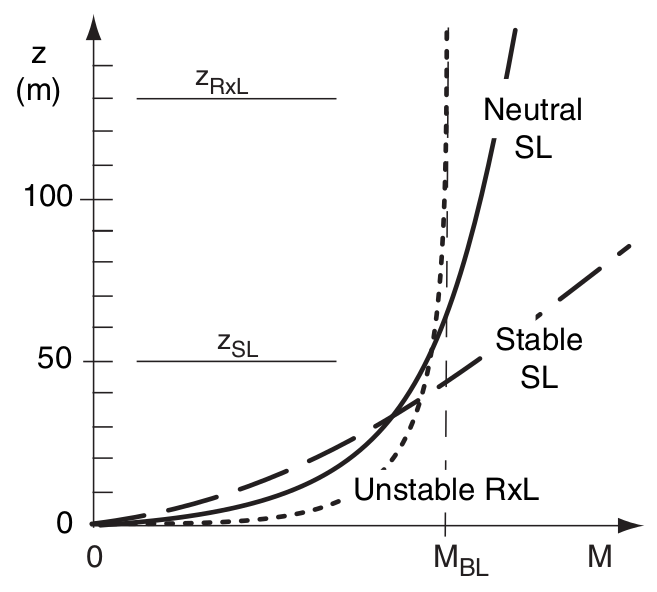
\includegraphics[width=\textwidth]{img/SL_wind.png}  
%@   %Fig 18.20 Stull
%@    %\begin{center}
%@    %\begin{tikzpicture}
%@    %  
%@    %\end{tikzpicture}
%@    %\end{center}
%@\end{columns}
%@ \footnote{donde: $u_*$: velocidad de fricción. $z_0$: coeficiente de rugosidad. $L$: longitud de Monin-Obukhov. $w_*$: Velocidad convectiva.}   
%@\end{frame}
%@
%@
%@
%@
%@\begin{frame}{Longitud de Monin-Obukhov}
%@
%@    Representa la altura (en metros) sobre la cual la producción mecánica de turbulenta es balanceada con la producción de empuje térmico.
%@    $$\boxed{
%@        L=\dfrac{-\rho \,c_p\,T_a\,u_*^3 }{g\,\kappa\,H}
%@        }
%@    $$
%@ 
%@ Está estrechamente vinculado a la estabilidad atmosférica:
%@    \begin{itemize}
%@        \item Estable: $L > 0$ %(since H < 0) very stable: 0 < L < 10
%@        \item Inestable: $L < 0$ %(since H > 0) 
%@        %very unstable: -10 < L < 0
%@        \item Neutra $|L| > 1000$
%@    \end{itemize}
%@    
%@\end{frame}
%@
%@\begin{frame}{Velocidad convectiva}
%@
%@Relacionado a la velocidad vertical de grandes térmicas (remolinos convectivos)
%@
%@Depende de:
%@\begin{itemize}
%@    \item Magnitud de la energia turbulenta convectiva
%@    \item Longitud de escala para los remolinos (i.e. altura de capa de mezcla: $z_i$ )
%@\end{itemize}
%@ 
%@$$\boxed{
%@w_*=\bigg( \dfrac{g\,z_i\,H}{c_p\,\rho\,\theta}\bigg)^{1/3}
%@}
%@$$
%@
%@Valores en el orden de 1-2 m/s
%@
%@\end{frame}
%@
%@
%@
%@\section{Altura de capa de mezcla}
%@
%@\begin{frame}{Altura de capa de mezcla}
%@
%@La altura de capa de mezcla está determinada por dos procesos, los esfuerzos de corte y la convecciòn. Este último solo es importante en atmósferas inestables.
%@    %\begin{figure}
%@    %    \centering
%@    %    \includegraphics[width=0.2\textwidth]{img/scaleHeights.png}
%@    %    \caption{Caption}
%@    %\end{figure}
%@    \begin{center}
%@    \begin{tikzpicture}[scale=0.8, random/.style={decorate,decoration={random steps,amplitude=2pt}}]
%@    \begin{scope}[xshift=-3cm, black!80]
%@       \piso{-2}{2}{0.1}
%@       \draw[random] (-2,2) -- (2,2);
%@       
%@       \draw[latex-latex,xshift=-0.2cm] (-2,0)--(-2,2) node[midway, anchor=east]{$z_{im}$};
%@       
%@       \draw[-latex, very thick] (-0.5,1)--(0.5,1)node[midway,above]{$u_*$};
%@       \node at (0,-0.5) {Estable};
%@    \end{scope} 
%@    
%@    \pause
%@     
%@    \begin{scope}[xshift= 3cm,black!80]
%@      \piso{-2}{2}{0.1}
%@      \draw[random] (-2,2) -- (2,2);
%@      \draw[random] (-2,5) -- (2,5);
%@    
%@      \draw[latex-latex,xshift=0.2cm] ( 2,0)--( 2,5) node[midway, anchor=west]{$z_{ic}$};
%@      
%@      %\node at (0,1){$u_*$};
%@      \draw[-latex, very thick] (-0.5,1)--(0.5,1)node[midway,above]{$u_*$};
%@      \node at (0,3.3){$w_*$};
%@      \node at (0,-0.5) {Inestable};
%@      
%@      \draw[->] (-1.2,2.3) to[out=10,in=-90] (-0.5 ,4.3);
%@      \draw[->] ( 1.2,2.3) to[out=170,in=-90] (0.5 ,4.3);
%@    \end{scope} 
%@    \end{tikzpicture}
%@    \end{center}
%@    
%@Decimos que hay convección \alert{forzada} en el primer caso, y convecciòn \alert{libre} en el segundo.
%@    
%@\end{frame}
%@
%@\begin{frame}{Altura de capa de mezcla}
%@ 
%@Considerando el mezclado \alert{turbulento mecánico}:
%@    $$
%@   \text{En condiciones neutrales:}\qquad  h_{\text{mix}}=\dfrac{0.3 u_*}{|f|}
%@    $$
%@    $$\text{En condiciones estables:}\qquad
%@    h_{\text{mix}}=C\sqrt{\dfrac{ u_* L}{|f|}  }
%@    $$
%@    
%@Bajo condiciones inestables, la $h_{\text{mix}}$ esta principalmente determinada por \alert{mezclado térmico}:
%@    $$\text{En condiciones inestables:}\qquad
%@    h_{\text{mix}}\approx D\sqrt{\dfrac{ u^3_*}{|f|^3L}  }
%@    $$
%@ 
%@\end{frame}
%@

%\section{Turbulencia}
%\begin{frame}{Turbulencia}
%    
%\textit{La turbulencia es parte del flujo no principal que experimenta variaciones abruptas, irregulares, y caóticas.}\\[0.5em]
%
% 
%Es un fenómeno multi-escala, casi exclusivamente tridimensional, de estado transitorio y que  produce \alert{mezcla}.\\[0.5em]
%
%La turbulencia \textbf{no} es una magnitud que se conserva:
%\begin{itemize}
%    \item Es disipada por la \textbf{viscosidad}.
%    \item Es producida y mantenida por: \alert{convección} y \alert{esfuerzos de corte}
%\end{itemize}
%
%
%La turbulencia \textbf{no} se modela, pero sí se estima su contribución a los flujos atmosféricos. 
%Si bien es un fenómeno deterministico, al ser caótico, es común utilizar aproximaciones \alert{estadísticas} para su estudio y modelación.
%
%\end{frame}
%
%\begin{frame}{Turbulencia}{Descomposición de Reynolds}
%
%$$u = \overline{u}+u' $$
%
%\begin{center}
%%\includegraphics[width=0.5\textwidth]{img/reynolds.png}
%\begin{tikzpicture}[scale=0.8]
%\begin{axis}[xshift=-5cm,xlabel=$t$,ylabel=$u$,xmin=0,xmax=8,ymin=-2,ymax=2]
%\addplot[domain=0:8,blue,samples=126,line width=0.7pt] expression{0.01*x+sin(90*x)+0.4*rand};
%\draw[dashed] (0,0)--(3,0)node[above]{$\overline{u}$}--(8,0);
%\draw[<->](5,0)--(5,0.9) node[midway,right]{$u'$};
%\end{axis}
%\end{tikzpicture}
%\end{center}
%
%\end{frame}   
%
%
%\begin{frame}{Turbulencia}{Medidas de turbulencia}
%
%Definición de promedio:
%$$ \overline{u}=\frac{1}{N}\sum_{i=1}^{N} u_i $$
%
%Variancia de velocidad del viento: 
%$$ \sigma_u^2 = \frac{1}{N}\sum_{i=1}^N (\alert{\overline{u} - u_i} )^2$$
%
%Por lo tanto:
%$$ \sigma_u^2= \overline{\alert{u'}^2} $$
%
%Tambien se puede elegir la variancia de otras variables (temperatura, presión, etc.).
%
%
%\end{frame}
%%
%%\setbeamercolor{background canvas}{bg=yellow!10}
%%
%\begin{frame}{Turbulencia}{Turbulent Kinetic Energy (TKE)}
%
%$$
%k = \frac{1}{2} \bigg[ { \sigma_u^2+ \sigma_v^2 + \sigma_w^2} \bigg]
%$$
%
%
%
%$${\displaystyle \underbrace {\frac {\partial k}{\partial t}} _{\begin{smallmatrix}{\text{Local}}\\{\text{derivative}}\end{smallmatrix}}+\underbrace {{\overline {u}}_{j}{\frac {\partial k}{\partial x_{j}}}} _{\begin{smallmatrix}{\text{Advection}}\end{smallmatrix}}=-\underbrace {{\frac {1}{\rho _{o}}}{\frac {\partial {\overline {u'_{i}p'}}}{\partial x_{i}}}} _{\begin{smallmatrix}{\text{Pressure}}\\{\text{diffusion}}\end{smallmatrix}}-\underbrace {{\frac {1}{2}}{\frac {\partial {\overline {u_{j}'u_{j}'u_{i}'}}}{\partial x_{i}}}} _{\begin{smallmatrix}{\text{Turbulent}}\\{\text{transport}}\\{\mathcal {T}}\end{smallmatrix}}+\underbrace {\nu {\frac {\partial ^{2}k}{\partial x_{j}^{2}}}} _{\begin{smallmatrix}{\text{Molecular}}\\{\text{viscous}}\\{\text{transport}}\end{smallmatrix}}\underbrace {-{\overline {u'_{i}u'_{j}}}{\frac {\partial {\overline {u_{i}}}}{\partial x_{j}}}} _{\begin{smallmatrix}{\text{Production}}\\{\mathcal {P}}\end{smallmatrix}}-\underbrace {\nu {\overline {{\frac {\partial u'_{i}}{\partial x_{j}}}{\frac {\partial u'_{i}}{\partial x_{j}}}}}} _{\begin{smallmatrix}{\text{Dissipation}}\\\varepsilon _{k}\end{smallmatrix}}-\underbrace {{\frac {g}{\rho _{o}}}{\overline {\rho 'u'_{i}}}\delta _{i3}} _{\begin{smallmatrix}{\text{Buoyancy flux}}\\b\end{smallmatrix}}}$$
%
%
%%$$
%%\dfrac{\partial k}{\partial t} = \vec{v} \cdot \nabla e + u_*^2 \dfrac{\partial u}{\partial z} + \dfrac{|g|}{T_v}\, H + \varepsilon
%%$$
%
%Convección:
%\begin{itemize}
%    \item Libre: Si $|b| < |\mathcal {P}/3| $
%    \item Forzada Si $|b| > |3\,\mathcal {P}|$
%\end{itemize}
%
%\end{frame}
%
%
%\begin{frame}{Turbulencia}{Número de \alert{Richardson}}
%
%%STULL: The ratio of buoyant energy to shear-kinetic energy is called the bulk Richardson number , Riwhich is dimensionless:
%%JACOBSON: give the ratio of turbulence due to buoyancy relative to that due to shear.
%Es un numero adimensional que mide la relación entre la turbulencia debido a flotación (convectiva) y debido a esfuerzos de corte (mecánica):
%
%$$
%\text{Ri}=\frac{ \text{flotacion}}{\text{esfuerzo cortante}}=\frac{g}{\rho}\frac{\partial \rho /\partial z}{(\partial u/\partial z)^{2}}
%$$
%
%Una versión discretizada muy utilizada es el \alert{Bulk Richardson Number}:
%
%$$
%{\displaystyle R_{B}={\frac {(g/T_{v})\Delta \theta _{v}\Delta z}{(\Delta U)^{2}+(\Delta V)^{2}}}}
%$$
%
%\end{frame}
%
%
%\begin{frame}{Turbulencia}{Covarianza y autocorrelación}
%% Varianza:
%% $$ \mathit{var}(u) = \frac{1}{N} \sum_{i=1}^{N} (u_i -\overline{u})^2$$
% 
% Podemos calcular la covariancia entre dos variables:
%% $$
%\begin{align*}%{ll}
%\mathit{covar}(u,\theta) &= \frac{1}{N} \sum_{i=1}^{N} (u_i -\overline{u})\,(\theta_i -\overline{\theta})\\
%&=\frac{1}{N} \sum_{i=1}^{N} u_i'\,\theta_i' \\
%&= \overline{u'\theta'} 
%\end{align*}
%%$$
%\end{frame}
%
%\begin{frame}{Turbulencia}{Covariancia}
%
%La covarianza mide la cantidad de variación común entre dos variables. 
%
%\begin{tikzpicture}[scale=0.7]
%\begin{axis}[xshift=-5cm,xlabel=$t$,ylabel=$x(t)$,xmin=0,xmax=8,ymin=-2,ymax=2]%Ç,grid=major,grid style={solid}]
%\addplot[domain=0:8,blue,samples=126,line width=0.7pt] expression{-0.4+0.2*x+sin(90*x)+0.4*rand};
%\addplot[domain=0:8,orange!80,samples=126,line width=0.7pt] expression{-0.4+0.2*x+sin(90*x+0.01)+0.4*rand-0.7};
%\end{axis}
%\begin{axis}[xshift=5cm,xlabel=$t$,ylabel=$x(t)$,xmin=0,xmax=8,ymin=-2,ymax=2]%Ç,grid=major,grid style={solid}]
%\addplot[domain=0:8,blue,samples=126,line width=0.7pt] expression{0.2*x+sin(90*x)+0.4*rand};
%\addplot[domain=0:8,orange!80,samples=126,line width=0.7pt] expression{-0.5-(0.2*x+sin(90*x+0.01)+0.4*rand-0.7)};
%\end{axis}
%\end{tikzpicture}
%
%Es positivo si ambas variabeles crecen/decrecen conjuntamente. Es negativa si la variación es opuesta/inversa. Y es cercana a cero si son independientes. 
%
%\end{frame}
%
%%\begin{frame}{Turbulencia}{}
%%
%%Coeficiente de correlación
%%$$ r(u,\theta)= \dfrac{\overline{u'\,\theta'}}{\sigma_u\,\sigma_\theta}$$
%%
%%Es una normalización de la covariación. Vale 1 para variables perfectamente correlacionadas, -1 para variables inversamente-correlacionadas y 0 para variables independientes.
%%
%%\end{frame}
%
%
%\begin{frame}{Turbulencia}{Covarianza y flujos turbulentos}
%    
%    Las covarianzas representan \textbf{ flujos turbulentos}!
%    \begin{center}
%        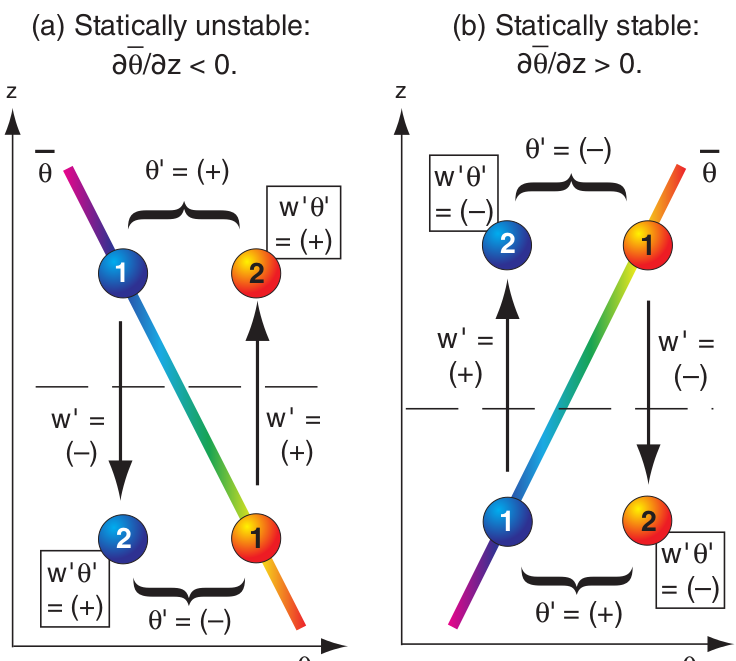
\includegraphics[width=0.4\textwidth]{img/covar_flujo.png}
%    \end{center}
%    
%    $$ \overline{w'\theta'}= F_{H} $$
%    
%\end{frame}
%

%===================================================================================
%SIMILITUD

%\section{Similitud}
%\begin{frame}{Similitud}{}
% 
%Asume que todas las atmósferas se comportan escencialmente de la misma forma pero a distintas escalas.
%Uno de los métodos para construir relaciones entre variables es el \textit{análisis dimensional}. 
% 
%\begin{block}{Teoréma $\pi$ de Buckinham:}
%Dado una problema descrito por un conjunto de ecuaciones de $k$ variables, con $p$ magnitudes fundamentales. Podemos definir $n$ valores adimensionales. Donde:
%$$n= k - p$$
%\end{block}
% 
%\end{frame}
%   
%\begin{frame}{Similitud}
%    Variables que describen el flujo en la capa lìmite: ($u$,$z$,$\rho$,$\nu$,$\tau$)
%    \footnote{ donde        $u$: velocidad del viento,        $z$: altura, $\rho$: densidad del aire, $\nu$: viscosidad (despreciable en régimen turbulento), $\tau$: esfuerzo de corte.}
%    Consideramos $\nu$ despreciable, y definimos la variable \textbf{velocidad de fricción} como:
%    $$ u_* = \sqrt{\frac{|\tau|}{\rho}}$$
%    reduciendo el número de variables a ($u$,$z$,$u_*$), con dos dimensiones, usando el teorema $\pi$-de Buckingham:
%    $$ \pi=\dfrac{z}{u_*}\dfrac{du}{dz}= \text{cte.} = \dfrac{1}{\kappa} \quad\Rightarrow\quad  du = \dfrac{u_*}{\kappa}\dfrac{dz}{z}$$
%    
%    Integrando y despejando $u$ obtenemos:
%    $$ u = \dfrac{u_*}{k} (\ln z + cte.)$$
%    
%\end{frame}
% 
% 
%\begin{frame}{Capa limite}{Perfil de velocidad de viento}
% 
%\begin{itemize}
%    \item Superficie plana, condiciones adiabaticas (neutral):
%    $$ u = \dfrac{u_*}{k} (\ln z + cte.)$$
%    
%    \item Superficie rugosa, condiciones neutral:\footnote{$z_0$: rugosidad de la superficie. Representa la altura extrapolada donde $u=0$}. Asumiendo que $u$ depende de $z/\varepsilon$
%    $$ u = \dfrac{u_*}{k} \bigg[ \ln \dfrac{z}{\varepsilon} - \ln \dfrac{z_0}{\varepsilon} \bigg] \quad\Rightarrow\quad u = \dfrac{u_*}{k} \ln \dfrac{z}{z_0} $$
%    
%%    \item Superficie rugosa, condiciones no neutrales:    
%%    $$ u = \dfrac{u_*}{k} \bigg( \ln \frac{z}{z_0} + 5 \dfrac{z-z_0}{L} \bigg)$$
%\end{itemize}
% 
%\end{frame}
% 
% 
%\begin{frame}{Capa límite}{Perfil de velocidad de viento, Monin-Obukhov}
% 
%Proponen agregar un factor de corrección por calentamiento de la superficie: $\phi(\xi)$ que depende de la estabilidad ($\xi$)
%\begin{columns}
% \column{0.5\textwidth}
% 
%$$
%\dfrac{\kappa z}{u_*}\dfrac{\partial u}{\partial z} = \phi(\xi)
%$$
% 
%Experimentalmente se vio que: 
%$$ \phi(\xi) =\begin{cases}
%    1+4.7 \xi        & \xi > 0  \\
%    1                & \xi = 0  \\
%    (1-15\xi)^{1/4}  & \xi < 0  \\
%\end{cases} 
%$$
% \column{0.5\textwidth}
%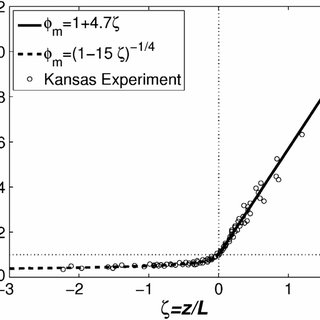
\includegraphics[width=0.7\textwidth]{img/kansas_experiment.jpg}
%\end{columns}
%\end{frame}
% 
% 
%\begin{frame}{Capa límite}{Longitud de Monin-Obukhov}
%El perfil de vientos depende fuertemente de la estabilidad atmosférica. Un indicador de estabilidad propuesto es:
%$$\xi =\dfrac{k\,g\,z \,H}{\rho_0\,c_p\,T_0 \,u_*^3} $$
% 
%depende de $z$, lo que es incombeniente, por eso se definió 
%$$L=z/\xi$$
%por lo tanto:
%$$L =\dfrac{\rho_0\,c_p\,T_0 \,u_*^3}{k\,g\, H} $$
%    
%\end{frame}
% 
% 
% 
% 
%\begin{frame}{Capa límite}{Perfil de velocidad de viento, Monin-Obukhov}
%$$   
%du = \dfrac{u_*}{\kappa} \phi(\xi) \dfrac{dz}{z}
%$$
% 
%Si $\xi > 0$ (estables) hay solución analítica:  
%    $$ u = \dfrac{u_*}{k} \bigg( \ln \frac{z}{z_0} + 5 \dfrac{z-z_0}{L} \bigg)$$
% 
%Para $xi < 0$ (inestable) no hay solución analítica exacta, pero se conoce una aproximación (Benoit, 1977):\footnote{donde $n_0=(1-16z_0/L)^{1/4}$  y $n=(1-16z/L)^{1/4}$}
% 
%$$
%u= \dfrac{u_*}{\kappa} \bigg\{  \ln \frac{z}{z_0} + \ln \bigg[\dfrac{(n_0^2 + 1) \,(n_0 +1)^2}{(n^2 + 1) \,(n +1)^2} \bigg] + 2 [\arctan n - \arctan n_0 ]\bigg\}
%$$
% 
%\end{frame}
% 
% 
% 
% 
% 
% 
% 
% 
% 
% 
% 
% 
% 
% 
% 
%\begin{frame}{Capa límite}{Perfil de temperatura}
% 
%Podemos definir la temperatura potencial de fricción como:
%$$ \theta_* = - \dfrac{H}{\rho c_p u_*}$$
% 
%Escribiendo $L$ en términos de $\theta_*$:
%$$ L = \dfrac{u_*^2\,T_0 }{\kappa \,g\,\theta_*}$$
% 
%De forma análoga a la velocidad se puede calcular los perfiles de temperatura.
% 
%\end{frame}
% 
% 
%\begin{frame}{Balance de calor}{Bajo condiciones estables}
% 
%De la definición de $\theta_*$:
%$$ H = - \rho c_p u_* \theta_* $$
% 
%$$ \theta_* = 0.009(1-0.5n^2)$$
% 
%$$ u = \dfrac{u_*}{k} \bigg( \ln \frac{z}{z_0} + 5 \dfrac{z-z_0}{L} \bigg) = \dfrac{u_*}{k} \bigg( \ln \frac{z}{z_0} + 5 \kappa g \theta_* \dfrac{z-z_0}{T u_*^2} \bigg) $$
% 
%Reordeno, multiplico por $\kappa u_* / \ln(z/z_0)$ y llego a:\footnote{donde $C_D= \kappa / \ln(z/z_0)$}
% 
%$$
%u_*^2 - C_D u \,u_* + C_D u^2 = 0
%$$
%Resuelvo la cuadratica para $u_*$:
% 
%$$
%u_* = \dfrac{C_d u}{2}\bigg[   1 + \sqrt{ \bigg( \dfrac{2\, u}{\sqrt{C_D} u }\bigg)^2 } \bigg]
%$$
% 
%\end{frame}


%\begin{frame}{Turbulencia}{Similitud}
%
%Variables utilziadas en analisis dimensional: ($\sigma_u$,$u_*$,$L$,$h_{\text{mix}}$, $z$). 
%
%En \alert{condiciones neutras ó estables},
%$$\sigma_u = u_* 2.5 \bigg(  1- \dfrac{z}{h_{\text{mix}}}   \bigg)^a
%\qquad
%\sigma_v = u_* 1.9 \bigg(  1- \dfrac{z}{h_{\text{mix}}}   \bigg)^a
%\qquad
%\sigma_w = u_* 1.3 \bigg(  1- \dfrac{z}{h_{\text{mix}}}   \bigg)^a
%$$
%
%En \alert{condiciones inestables}, se define una nueva velocidad de escala convectiva ($w_*$) para contemplar la turbulencia inducida termicamente:
%
%$$ w_* = \bigg( \dfrac{g\,z_i\,H}{c_p\,\rho\,\theta} \bigg) \quad\Rightarrow\quad w_* = \bigg( \dfrac{h_{\text{mix}}}{L\,\kappa}\bigg)^{1/3} $$
%
%Por debajo de la capa de mezcla se obtiene experimentalmente:
%
%$$
%\dfrac{\sigma_u}{w_*}=\dfrac{\sigma_u}{w_*}=\dfrac{\sigma_u}{w_*}=0.6
%$$
% Independientemente de la altura. Por encima de la capa de mezcla la turbulencia decae exponencialmente.
%\end{frame}

%% FIN SIMILITUD
%==============================================================================================